TODO: Describe how we optimized OpenNebula (move relevant content from previous section here)

The startup times for each cluster deployment varied and the most representative ones are those obtained for the larger deployment, the 101 node cluster. In this case, the time needed by the rOCCI client to return all the resource endpoints corresponding to each VM ranged from 71 to 86 minutes. This is just the time to get the identifier corresponding to each VM instance, actually to have all the VMs running took even longer, around 80 minutes more. So the total cluster startup time ranged from 2.5 to 3 hours. But this was not the main issue encountered, the main problem was that some of the rOCCI requests failed with an \emph{execution expired} error and some of the VMs did not start--in the worst case 21 out of 101 failed.
%\begin{verbatim}
%An error occurred! Message: execution expired
%An error occurred! Message: HTTP Response status: [500] Internal Server Error!
%\end{verbatim}
We started to see this type of errors as soon as we tried to deploy, in a sequential way, more than 20 VMs at CESGA. In CESNET we could not do this analysis because there were only 10 VM slots available due to a restriction in the amount of public IPs that they had available.

Trying to understand the source of this issue we tracked the performance of the OpenNebula frontend during the cluster startup. As it can be seen in Figure \ref{fig:on} the frontend experiences a high load several minutes after the start of the cluster deployment, this causes it to respond slower, probably producing the rOCCI execution expiration errors mentioned above. Looking at the processes in the OpenNebula frontend, we could see that this increase in the load is mainly due to the scp processes launched to copy the image template to the OpenNebula nodes, more than 20 simultaneous scp processes seem to affect considerably the system performance, reducing its response times considerably.

% * Deploying 101 VMs:
%{{{
%[jlopez@test13 ~]$ time ./deploy_cluster_voms.sh &> deploy_cluster_voms.log
%
%real	71m31.677s
%user	1m43.104s
%sys	0m25.706s
%
%[jlopez@test13 ~]$ wc -l machines/pending
%98 machines/pending
%
%}}}
%

% Screenshot ganglia: 100 VMs deployment
\begin{figure}[t!]
\centering
%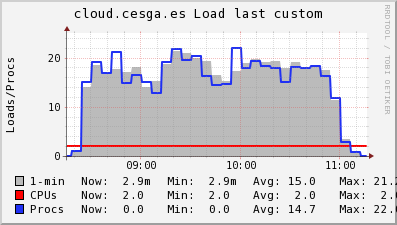
\includegraphics[width=0.74\textwidth]{figures/ON_load-complete.png}
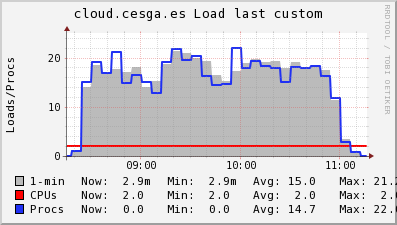
\includegraphics[width=0.6\textwidth]{figures/ON_load-complete.png}
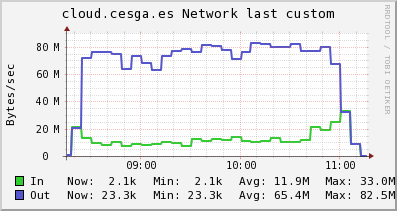
\includegraphics[width=0.6\textwidth]{figures/ON_network-complete.png}
\caption{OpenNebula frontend load and network usage graphs taken from Ganglia during the deployment of the 101 nodes cluster.}
\label{fig:on}
\end{figure}


Another problem we encountered was that FedCloud does not count with a workload management system, so each VM creation request must be sent to the appropriate endpoint. This means that we have to take care in advance of the partitioning of the cluster between the different FedCloud sites. In our case we choose to run 10 VM at CESNET--the maximum possible at the time of the benchmarks--and the rest of them at CESGA--ranging from 10 to 91.

Once the cluster is deployed we proceed to configure Hadoop. In this case the only problem encountered was due to the global firewall rules at each site that blocked Hadoop communications. Once this issue was addressed the Hadoop cluster started flawlessly. The time involved to configure and start the Hadoop cluster was really short, taking less than 1 minute in the larger setup with 101 nodes, so it is almost irrelevant in the total cluster startup time when considering the almost 3 hours needed for VM instantiation.

The optimized startup times can be found in Table \ref{table:startupON}.

%% Table startup Amazon EC2
\begin{table}[h!]
\caption{Amazon EC2 startup times using our custom tool (available at github): the AMI used was eu-west-1/ami-54d43023 EBS plus instance store. The instance type used was m1.small in all cases.}
\label{table:ec2}
%
\vspace{-0.5em}
%
\begin{center}
\begin{tabular}{ccl}
\toprule
Cluster size			& Startup time (s)	& Comments	  \\
\midrule
10                		& 191   		&	 \\
21                   		& 178			&        \\
51                   		& 583*			& 2 nodes not working       \\
101                  		& 276*			& 16 nodes not working       \\
101                  		& 297*			& 1 node not working       \\
%
\bottomrule
\multicolumn{3}{c}{\rule{0.98\textwidth}{0em}}\\
\rule{0.2\textwidth}{0cm} & \rule{0.2\textwidth}{0cm} &  \\
\end{tabular}
\end{center}
%\vspace{-3.5em}
%\tablenotetext[a] {Identifies the configuration file where the parameter is set, the complete configuration files can be found at \url{https://github.com/grid-admin/hadoop}}
\end{table}

